\chapter{Approach}

\section{Solution Strategy} 

This project’s goal is to distinguish contrails from the clouds, so we start 
by investigating the main difference between contrails and clouds. 

Contrails usually show as a line on an image. Meanwhile, the clouds 
exhibit a random discrete distribution. Knowing this, we write a program 
to detect the straight lines in images to recognize the contrails. 

However, it should be realized that even when the contrails look like pencil 
lines on the image, there actually doesn’t exist an actual straight line 
when looking through the image data. Contrails also have some width in 
the image (in the real world, contrails could be several kilometers in width 
[CONTRAILS FACTS, page 3]). The real shape of contrails seems more like 
some long and thin rectangles with two fading sides. In this case, the 
detection problem became much harder. 

Since this solution is hard to compute, instead of detecting the contrails’ widths, 
it is much easier to just detect the two clear sides of contrails. In this case, 
we can ignore the image inside the contrails, as well as other pixels inside 
the cloud by doing the edge detection.

After performing edge detection to detect edgels (pixels that are edge elements), 
we can detect lines using the Hough Transform on the edgel map. Another problem 
was that there were too many edgels in the image (see the results in
Figure \ref{fig_edgels} below). Those bad edgels can cause to the Hough Transform 
to give incorrect lines, which do not come from contrails.

To solve this problem, some preprocessing on the edgel maps to get rid of 
bad edgel is necessary. In order to delete those bad edgels from clouds 
or other graphics, each pixel in a specific neighbouthood is
checked as a small block. Because lines can be divided into an infinity of
small lines, if a line goes through a small block, there must exist a small 
line inside the small block. We can use polynomial curve fitting to get 
the slope of the best small line in each block. Then we check how well 
the block edgels fit the computed line. Poor fits, as determined by a 
line residue, causes an edgel at the center of the neighbourhood
to be rejected from the further Hough Transform.

After this preprocessing, I use the Hough Transform and obtain
a much better line detection result.

The complete algorithm:
\begin{enumerate}
    \item Convert the color image to a grayvalue image;
    \item Use the Canny edge detection to compuyte the edge map of the grayvalue image;
    \item Using the neighbouthoods about each edgel (left to right, top to bottom) 
          we perform polynomial curve fitting to get the best small line 
          information (slope and intercept);
    \item Put all the edgels surviving the polynomial curve fitting procedure 
          into a new image;
    \item Perform the Hough Transform on the new image;
    \item Median filter the new image;
    \item Plot the results.
\end{enumerate}

\section{MatLab Methods}

The MatLab code for Canny edge detection is given in the subsection below.

\subsection{Canny Edge Detection}
\vspace{3mm}
\textit{Edge\_image = edge (I, \lq{canny}\rq);}\\
\textbf{Input: I, grayscale Image}\\
\textbf{Output: Edge\_image, the black and white edge image}\\
\newline
Canny edge detection is a technique for extracting useful structural 
information from different visual objects and dramatically reducing 
the amount of data to be processed. These are following steps:
\begin{enumerate}
\item Apply Gaussian filtering to remove noise;
\item Compute the intensity gradient of the image;
\item Apply non-maximum suppression to get rid of spurious responses to edge detection;
\item Apply a double threshold to determine potential edges to filter out the 
edgels with a weak gradient value and preserve edgels with high gradient values;
\item Track edges using hysteresis: Finalize the detection of edges by suppressing 
all the other edges that are weak and not connected to strong edges.
\end{enumerate}


\subsection{Polynomial curve fitting}

Again we use MatLab to fit polynomials to the edgel images.
\vspace{3mm}
\textit{p = polyfit(x,y,n);}\\
\newline
\textbf{Input: \\x and y, vectors containing the x and y data to be fitted;\\ n, the degree of the polynomial to return;}\\ 
\textbf{Output: p, the third-degree polynomial that approximately fits the data.}\\
\newline
This algorithm returns the coefficients for a polynomial $p(x)$ of degree $n$ 
that is the best fit (in a least-squares sense) for the data in $y$. The 
coefficients in $p$ are in descending powers and the length of $p$ is $n+1$.


\subsection{Hough Transform and Hough Line Transform}

We show the MatLab for the Hough transform below.

\begin{wrapfigure}{r}{5.5cm}
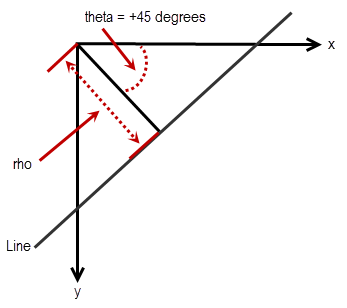
\includegraphics[width=5cm]{pic/SHT-example.png}\\
\caption{theta($\theta$) and rho($\rho$) of Hough Transform}
\label{fig1}
\end{wrapfigure}
\vspace{3mm}
\textit{[H,theta,rho] = hough(BW);}\\
\newline
\textbf{Input: BW, the black and white image;}\\
\textbf{Output:\\ H, the Hough Transform matrix be returned as a numeric array;}\\ 
\textbf{theta($\theta$), the angle in degree between the x-axis and rho vector;}\\
\textbf{rho($\rho$), the distance from origin to the line along a vector perpendicular to the line;}\\

The Standard Hough Transform (SHT) uses the parametric representation of a line: 
\begin{equation}
\rho = x cos(\theta) + y sin(\theta).
\label{eqn_parametric}
\end{equation} 
For each edgel in the image, the numbers of lines going through it 
with all different angles is large. If 2 edgels are on the same line, 
they have the same $\rho$ and $\theta$ valuesr. In a graph of the
different angle and distances from the origin, the $\rho$ and $\theta$
value copunts will be maximal.
\begin{figure}[ht]
    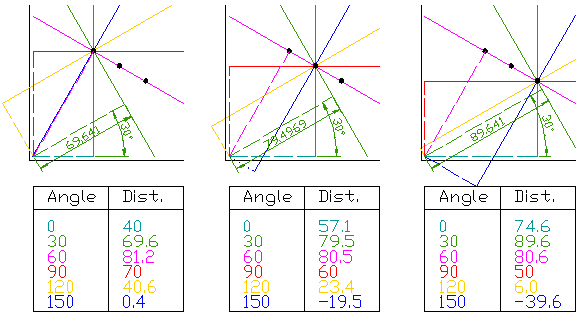
\includegraphics[scale=0.7]{pic/SHT-example2.png}
    \caption{$\theta=60^{\circ}$ and $\rho$ values are the same for the 3 points,
    see Wikipedia.com.}
\label{fig_SHT}
\end{figure}
As we can see from Figure \ref{fig_SHT}, when the Hough Transform algorithm 
goes through all different angles ($\theta$) for every edgel, there is a 
certain angle ($\theta=60^{\circ}$ in Figure \ref{fig_SHT}), that makes the 
perpendicular distance from the line to origin keeps the same 
$(\rho = 81.2 \approx 80.5 \approx 80.6)$. When we draw all the information 
below, we have a much clearer view of how the Hough Transform works.

\subsection{Median Filter}
We show how to do median filtering using MatLab.
\vspace{3mm}
\textit{B = medfilt2(A, [m n]);}\\
\newline
\textbf{Input:\\ A, the original image;}\\
\textbf{[m n], the isolate edgels’ size to be deleted;}\\ 
\textbf{Output: B, the image after deleted the isolated edgels.}\\
\newline
Median filtering works by puting the $m \times n$ edgels around each 
target edgel into an array and then sorting all the values in the array.
After this, we find the median value of the array and replace the target edgel
with that edgel.

\section{Algorithm to Reduce the Number of Bad Edgels}

\textbf{The input is an edgel image and the output 
is that edgel image with the small neighbourhoods containing small residual 
values deleted.}

Since Canny edge detection gives many edgels, we need to further process 
these edgel maps to eliminate edgels that are not parts of straight lines. 
For each $2\times s+1$ by $2\times s+1$ square neighborhood about an edgel
we fit all the neighborhood edgels to a straight line using polyfit. We 
fit either $y=mx+b$ for lines, where $\left|m\right| \leq 45^{\circ}$ and 
$x=\frac{y-b}{m}$, if $\left|m\right| \geq 45^{\circ}$. 
This takes care of horizontal and vertical lines. Now we have the equation 
of the best line fit for all the edgels in a neighborhood. But how good is 
this line fit? For each neighborhood edgel we compute the residual of that 
edgel’s neighborhood fit to the line. We compute the overall residual as 
the square root of the sum of these squared residual values.

Since neighbourhoods with poor line fits will have large overall residual 
values, we remove bad edgels using a threshold of 15, determined by trial and error.

\subsection{Pseudo code}

Here we present the pseudo code.
\begin{lstlisting}[language=Java]
I = Read image;
grayscale (I);
image = Canny edge detect(I);
set the block size, height and width (s, height, width)
	
initial number no lines = 0;

for x = (1+s) to (height-s):
    for y = (1+s) to (width-s):
    initial points number = 0:
        if pixel is on an edge:
            for i = (x-s) to (x+s):
                for j = (y-s) to (y+s):
        	        if block pixel is edge:
                        record them;
                        points number ++;
        	if at least one line in a block:
        	    m = polyfit (x and y data recoded);
        	    if (line’s slope >1 or <-1):
        	        compute the residual r;
        	    else:
        	        modify the m;
        	        compute the residual r;
        	    save r values
        	else:
                number no lines ++;
                
get non_zero_r;
sort non_zero_r;	
set the precentage p;
threshold = cast(p% * non_zero_r);


for x = (1+s) to (height-s):
    for y = (1+s) to (width-s):
        if the r value is in the shreshold and non zero:
	        write it on new_image;
	        
new_image = medfilter (new_image);
get Hough Transform matrix(H), theta(T) and rho(R) by hough(new_image);
get peaks(P) = houghpeaks (new_image);
lines = houghlines(new_image, T, R, P);

for k = 1 to number of lines:
    plot lines on origin image(I);

\end{lstlisting}
